\documentclass[a4paper,12pt]{article} % тип документа

\usepackage{tikz}
\usepackage[T2A]{fontenc}			% кодировка
\usepackage[utf8]{inputenc}			% кодировка исходного текста
\usepackage[english,russian]{babel}	% локализация и переносы
\usepackage{amsfonts,longtable}

% Математика
\usepackage{amsmath,amsfonts,amssymb,amsthm,mathtools} 


\usepackage{wasysym}

\title{Лабораторный журнал к работе 1.2.1 по курсу \\ "Общая физика"  \\ 
\vspace{0.2cm}
\vspace{4.5cm}
 \LARGE{\textbf{Определение скорости полета пули при помощи баллистического маятника}}\vspace{5.5cm}}
\date{12.10.2018}
\usepackage{tikz}
\author{\vspace{0.2cm}Баринов Леонид}

\begin{document}

\maketitle
\newpage

\textbf{Цель работы:} определить скорость полета пули, применяя законы сохранения и используя баллистические маятники.

\textbf{В работе используется:} духовое ружье на штативе, осветитель, оптическая система для измерения отклонений маятника, измирительная линейка, пули и весы для взвешивания, а также баллистические маятники.

\textbf{Теоритические данные:}
Для измерения переданного пулей импульса и, следовательно, ее скорости используют баллистический маятник. Баллитическим называется маятник, колебания которого вызываются кратковременныи начальным импульсом (толчком). Кратковременным можно считать импульс, если время действия сил (время соударения) значительно меньше периода колебаний маятника. При этом отклонение маятника за время соударения значительно меньше амплитуды колебаний - максимальное время соударения $\tau$, отнесенное к периоду колебаний $T$, и отклонение $\Delta\varphi$ за время соударения, отнесенное к максимальному отклонению $\Delta_m$ (амплитуде), связаны простым соотношением
\[\frac{\Delta\varphi}{\varphi_m}\approx\frac{2\pi\tau}{T}\]
Влияние струи газов на маятник можно оценить с помощью холостого выстрела. Ружье закреплено на специальном штативе. Чтобы зарядить ружье, надо освободить стопорный винт штатива и наклонить ружье в держателе набок. Затем отогнуть ствол в сторону курка до упора. Зарядив ружье, все вернуть в первоначальное состояние.
\begin{figure}[h]
\centering
\includegraphics[scale = 0.4]{1}
\caption{Схема установки для измерения скорости полета пули}
\end{figure}
\newpage
\textbf{Ход работы:}
\section{Метод баллистического маятника, совершающего поступательное движение}
Используемый в этой части работы баллистической маятник представляет собой тяжелый цилиндр, подвешенный на четерых нитях одинаковой длины. Он изображен на Рис. 1 вместе в измерительной системой.

Закон сохранения импульса при соударении пули с цилиндром имеет вид
\begin{equation}
mu = (M+m)V
\end{equation}
Здесь $m$ -- масса пули, $M$ -- масса цилиндра, $u$ -- скорость пули перед ударом, $V$ -- скорость цилиндра и пули после неупругого соударения.

Учитывая, что масса маятника значительно больше массы пули, можно написать
\begin{equation}
u = \frac{M}{u}V
\end{equation}
Получив начальную кинетическую энергию, маятник при отклонении будет подниматься до тех пор, пока всю ее не израсходует. Если пренебречь потерями, то вся кинетическая энергия переходит в потенциальную в поле тяжести. Тогда по закону сохранения механической энергии высота $h$ подъема маятника над его начальным положением связана с начальной скоростью маятника $V$ следующим образом:
\begin{equation}
V^2=2gh
\end{equation}
Здесь $g$ - ускорение свободного падения.

Высота подъема маятника выражается через угол $\varpi$ отклонения маятника от вертикали:
\begin{equation}
\begin{aligned}
h = L(1-cos\varphi) = 2Lsin^2\frac{\varphi}{2}, & & где \varphi\approx\frac{\Delta x}{L}\\
\end{aligned}
\end{equation}
Из (2), (3) и (4) получаем окончательную формулу для определения скорости пули:
\begin{equation}
u = \frac{M}{m}\sqrt{\frac{g}{l}}\Delta x
\end{equation}
\begin{figure}[h]
\centering
\includegraphics[scale = 0.4]{2}
\caption{Схема установки для измерения скорости полета пули}
\end{figure}
\begin{itemize}
\item Измеряем массу каждой пули на аналитических весах
\item Измеряем расстояние $L$
\item Собираем оптическую систему, предназначенную для измерения перемещения маятника. Включем осветитель и добиваемся четкого изображения шкалы на экране
\item Произведем несколько холостых выстрелов по маятнику и убеждаемя в том, что она практически не реагирует на удра воздушной струи из ружья.
\item Убедимся в малом затухании колебаний: за десть колебаний амплитуда уменьшается меньше, чем наполовину.
\item Произведем несколько выстрелов и определим по формуле (5) скорость пули при каждом выстреле.
\item Оценим погрешность определения скорости пули в каждом выстреле
\item Найдем среднее значение скорости пули в каждом выстреле.
\item Найдем среднее значение скорости пули и разброс отдельных результатов около среднего значения. 
\end{itemize}
\section{Метод крутильного баллистического маятника}
Схема эксперимента изображена на Рис. 3. Пуля массой $m$ попадает в мишень, укрепленную на стержне $aa$, который вместе с грузами $M$  и проволкой П образует крутильный маятник.
\begin{figure}[h]
\centering
\includegraphics[scale = 0.4]{3}
\caption{Схема установки для измерения скорости полета пули}
\end{figure}
 Считая удар пули о мишень неупругим, для определения скорости $u$ полета пули непосрдественно перед ударом воспользуемся законом сохранения момента импульса в виде
 \begin{equation}
 mur=I\Omega
 \end{equation}
 Здесь $r$ -- расстояние от линии полета пули до оси вращения маятника (до проволки П), $I$ -- момент инерции маятника, $\Omega$ -- его угловая скорость непосредственно после удара.
 
 Пренебрегая потерями, закон сохранения энергии при колебаниях записываем следующим образом:
 \begin{equation}
 k\frac{\varphi^2}{2}=I\frac{\Omega^2}{2}
 \end{equation}
 Здесь $k$ -- модуль кручения проволки П, а $\varphi$ -- максимальный угол поворота маятника.
 
Из (6) и (7) получаем
\begin{equation}
u = \varphi\frac{\sqrt{kI}}{mr}
\end{equation}
Угол максимального закручивания маятника в данных опытах всегда мал и легко находится по смещения $x$ изображения нити освитетля на измерительной шкале. Из Рис. 3 следует
\begin{equation}
\varphi\approx\frac{x}{2d}
\end{equation}
Здесь $d$ - расстояние от шкалы Ш до оси вращения маятника.

В формулу (8) входит проивзедения $kI$, которое можно найти по измерениям периодов колебаний мфятника с грузами $M$ и без них. В первом случае период колебаний равен:
\begin{equation}
T_1 = 2\pi\sqrt{\frac{I}{k}}
\end{equation}
Во втором случае
\begin{equation}
T_2 = 2\pi\sqrt{\frac{I-2MR^2}{k}}
\end{equation}
Из (10) и (11) следует
\begin{equation}
\sqrt{kI}=\frac{4\pi MR^2T_1}{T_1^2-T_2^2}
\end{equation}
Здесь $R$ -- расстояние от центров массс грузов $M$ до проволки.
\begin{itemize}
\item Измеряем на аналитических весах массу каждой из пулек
\item Измеряем с помощью линейки расстояние $r$, $R$ и $d$
\item Настроем оптическую систему, предназначенную для измерения проворота маятника. Включаем осветитель О, направим свет на зеркальце З и получаем четкое изображение нити осветителя на шкале.
\item Произведем несколько холостых выстрелов и убедимся, что маятник практически не реагирует на воздушную струю из ружья.
\item Убеждаемся в малом затухании колебаний: за десять колебаний амплитуда уменьшается меньше, чем наполовину.
\item Измеряя время 10-15 полных крутильных колебаний маятника, определяем $T_1$ и $T_2$. По формуле (12) найдем величину $\sqrt{kI}$ и оценим ее погрешность
\item Произведем несколько выстрелов и по формулам (9) и (8) определим скорость пули при каждом выстреле.
\item Оценим погрешность определения скорости пули в каждом выстреле.
\item Найдем среднее значение скорости пули и разброс отдельных результатов около срденего значения.
\end{itemize}
\newpage
\textbf{Экспериментальные данные:}

\textbf{ Метод баллистического маятника, совершающего поступательное движение}
\begin{table}[h]
\caption{Масса пуль}
\centering
\begin{tabular}{|c|p{2cm}|}
\hline
$\text{№}$ & $m$, кг \\ \hline
1 & \\ \hline
2 & \\ \hline
3& \\ \hline
4 & \\ \hline
\end{tabular}
\end{table}

Расстояние $L = $

\[u = \frac{M}{m}\sqrt{\frac{g}{l}}\Delta x\]
\begin{table}[h]
\centering
\caption{Измерение скорости пули в каждом выстреле и погрешность измерения}
\begin{tabular}{|c|p{2cm}|p{2cm}|}
\hline
$\text{№}$ & $u$, м/с & $\sigma$ \\ \hline
1 & &\\ \hline
2 & &\\ \hline
3& &\\ \hline
4 & &\\ \hline
\end{tabular}
\end{table}

$u_\text{ср}=$
\begin{table}[h]
\centering
\caption{Разброс отедльных результатов}
\begin{tabular}{|c|p{3cm}|}
\hline
$\text{№}$ & $|u-u_\text{cр}|$, м/с  \\ \hline
1 & \\ \hline
2 & \\ \hline
3& \\ \hline
4 & \\ \hline
\end{tabular}
\end{table}
\newpage
\textbf{Метод крутильного баллистического маятника}\\

$r = $\\

$R = $\\

$d =$\\

\begin{table}[h!]
\renewcommand{\tabcolsep}{3mm}
\centering
\caption{Измерение времени полных крутильных колебанмй маятника}
\label{table 4}
\begin{tabular}{|c|c|c|c|c|c|c|c|c|c|}
\hline
$\text{№}$ & 1 & 2 & 3 & 4 & 5 & 6  & 7 & 8 & 9\\ \hline
$T_1$, c&   &   &   &   &   &  &	&	& \\ \hline
$T_2$, c   &   &   &   &   &   &  &	&	&  \\ \hline \hline
$\text{№}$ & 10 & 11 & 12 & 13 & 14 & 15  & 16 & 17 & 18\\ \hline
$T_1$, c &    &   &   &   &   &  &	&	& \\ \hline
$T_2$, c   &   &   &   &   &   &  &	&	&  \\ \hline
\end{tabular}
\end{table}
$\sqrt{kI} = $
\\

$\sigma_{\sqrt{kI}}=$


\[u = \varphi\frac{\sqrt{kI}}{mr}\]

\[\varphi\approx\frac{x}{2d}\]


\begin{table}[h]
\centering
\caption{Измерение скорости пули в каждом выстреле и погрешность измерения}
\begin{tabular}{|c|p{2cm}|p{2cm}|}
\hline
$\text{№}$ & $u$, м/с & $\sigma$ \\ \hline
1 & &\\ \hline
2 & &\\ \hline
3& &\\ \hline
4 & &\\ \hline
\end{tabular}
\end{table}
$u_\text{ср}=$
\newpage
\begin{table}[h]
\centering
\caption{Разброс отедльных результатов}
\begin{tabular}{|c|p{3cm}|}
\hline
$\text{№}$ & $|u-u_\text{cр}|$, м/с  \\ \hline
1 & \\ \hline
2 & \\ \hline
3& \\ \hline
4 & \\ \hline
\end{tabular}
\end{table}
\end{document}